
\subsection{Einfeldt Strong Rarefaction Test}

This test measures the solver's vulnerability to very strong rarefactions that can, in some cases, 
produce negative mass densities or pressures. The input parameters can be tweaked slowly to determine 
exactly how strong the rarefaction can become before producing values that are NAN. 

The test was devised by Einfeldt to demonstrate the failure modes of many approximate Riemann solvers
used in Godunov methods.

\subsubsection{Initial Conditions}

Einfeldt's paper considers states lying in a 4-parameter region $\{ \rho, m, n, e \}$, with the
one-dimensional domain separated into $x > 0$ and $x < 0$. Imogen sets the box size to 1.

Initial conditions in Einfeldt's notation are:
\begin{itemize}
\item $\rho(x) = 1$
\item $\vec{v} = \{ sign(x) m, n, 0 \}$
\item $E_{\text{tot}} = e$
\end{itemize}
Einfeldt's original test is conducted for an adiabatic equation of state with index $\gamma = 7/5$.

Boundary conditions are constant for X.

Einfeldt's notation permits the entry of manifestly unphysical conditions (total energy < kinetic energy)
and care is therefore required.

Imogen's physical input parameters to the Einfeldt Strong Rarefaction test are:
\begin{itemize}
\item \tt{rho} - Defines the mass density of the whole region
\item \tt{m} - Defines the X-momentum of the region (parallel to the grid)
\item \tt{n} - Defines the Y-momentum of the region (perpendicular to the grid)
\item \tt{e} - Defines the energy density of the region
\end{itemize}

\subsubsection{Analysis}

\begin{figure*}
\begin{center}
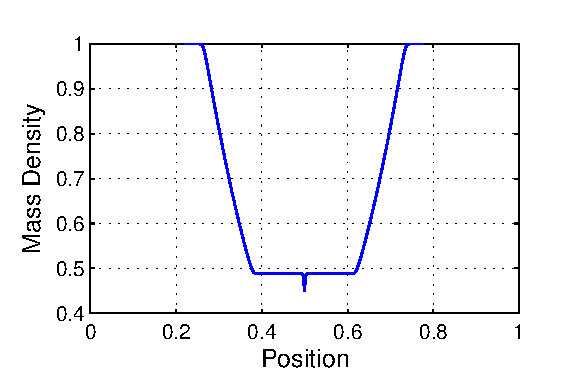
\includegraphics{Einfeldt.eps}
\caption{Einfeldt test at t = 0.1}
\end{center}
\end{figure*}

The evolution results in two rarefaction characteristics being emitted from the center of the
grid, and potentially a stationary region in the center.

For weak rarefactions, the solution contains six clearly defined regions:
\begin{itemize}
\item $x < -c_s t$ - farther left than leftgoing rarefaction fan
\item left rarefaction
\item left stationary region
\item right stationary region (separated by material contact)
\item right rarefaction fan
\item $x > c_s t$ - farther right than rightgoing rarefaction fan
\end{itemize}
As the Mach increases, the tails of the rarefaction fans move more and more slowly.
At a critical Mach number $M_*$ the middle stationary region vanishes. Above it,
the velocity profile becomes simple ($v = x / t, |x| < c_s t$) but the density profile
has proven difficult to solve (despite apparent simplicity).

